%
% Chapter 3
%
\chapter {Basics of Quantum Error Correction}

This chapter explains the basic concepts to understand how quantum computations can be performed reliably in the presence of noise. Given the fragility of coherent quantum systems, quantum error correction and fault-tolerant quantum computation are fundamental arbitrarily large quantum algorithms operating on many qubits.

\section{Noise and Error Correction}

Noise can introduce errors in data while it is being processed, sent through a channel and/or stored in a medium. A common error that can be introduced by noise is a bit flip (e.g. $0 \rightarrow 1$, $1 \rightarrow 0$). The task of error correction is to detect when an error has occurred and correct it.

In classical error correction, coding based on data-copying is extensively used. The key idea is to protect data against the effects of noise by adding redundancy. For example, a classical repetition code can encode a logical bit using three physical bits:
$$0 \rightarrow 000$$
$$1 \rightarrow 111$$

The problem is that classical error correction techniques cannot be directly applied to qubits because of the following reasons:
\begin{itemize}[noitemsep]
    \item It is impossible to create an independent and identical copy of a qubit in an arbitrary unknown state. This is known as the no-cloning theorem of quantum mechanics and it has the consequence that qubits cannot be protected from errors by simply making multiple copies\cite{NoCloningTheorem_1982}.
    \item Measurement destroys quantum information, implying that we cannot measure a qubit to decide which correcting action to perform.
    \item In addition to bit flip errors ($\ket{\psi}=\alpha\ket{0}+\beta\ket{1} \rightarrow \ket{\psi}=\alpha\ket{1}+\beta\ket{0}$), qubits are also susceptible to phase flip errors ($\ket{\psi}=\alpha\ket{0}+\beta\ket{1} \rightarrow \ket{\psi}=\alpha\ket{0}-\beta\ket{1}$) that have no classical analogous. Therefore, quantum error correction must be able to simultaneously correct for both.
    \item Errors in quantum information are continuous. This means that qubits, in the presence of noise, experience angular shifts rather than full bit or phase flips.
\end{itemize}

In order to protect qubits against the effects of noise, we can use the following process:
\begin{enumerate}[noitemsep]
    \item Encode: multiple physical qubits are used to encode a two-level quantum state into a logical qubit.
    \item Manipulation: operations are performed using the logical qubit (here's where errors can be introduced).
    \item Syndrome detection: measurements are performed that indicate what error, if any, ocurred.
    \item Recovery: the value of the syndrome is used to select the procedure to use to correct the error.
    \item Decode: logical qubit is decoded before final measurements are made.
\end{enumerate}

\section{Bit Flip Code}

To make it possible to correct bit flip errors, we can use three physical qubits to encode each logical qubit:
$$\ket{0_L}=\ket{000}$$
$$\ket{1_L}=\ket{111}$$
$$\ket{\psi}=\alpha\ket{0}+\beta\ket{1}  \underrightarrow{encode}  \ket{{\psi}_{L}}=\alpha\ket{0_L}+\beta\ket{1_L}$$

The notation $\ket{0_L}$ and $\ket{1_L}$ indicates that these are the logical $\ket{0}$ and logical $\ket{1}$ states, and not the physical $\ket{0}$ and physical $\ket{1}$ states.

A circuit that performs this encoding is illustrated in figure \ref{fig:BitFlipEncodingCircuit}:

\begin{figure}[h!]
    \centering
    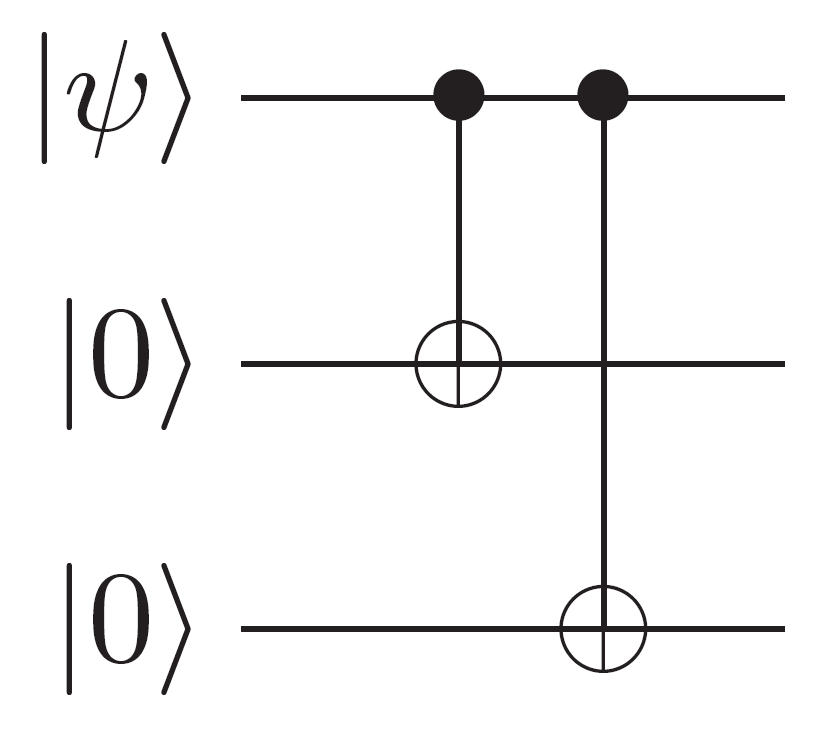
\includegraphics[scale=.25]{images/ErrorCorrection-BitFlipEncodingCircuit.png}
    \caption{Bit flip encoding circuit \cite{NielsenChuang_2012}}
    \label{fig:BitFlipEncodingCircuit}
\end{figure}

After the logical qubit has been manipulated, syndrome detection and recovery is done. There are four bit flip posibilities at this stage:
\begin{itemize}[noitemsep]
    \item No error: $\alpha\ket{000}+\beta\ket{111}$
    \item First qubit flipped: $\alpha\ket{100}+\beta\ket{011}$
    \item Second qubit flipped: $\alpha\ket{010}+\beta\ket{101}$
    \item Third qubit flipped: $\alpha\ket{001}+\beta\ket{110}$
\end{itemize}

For each one of these posibilities, the recovery operation is clear. The circuit shown in figure \ref{fig:BitFlipDetectionAndRecoveryCircuit} detects the error using two auxiliary qubits that are entangled with the logical qubit such that measurements on those qubits yield two classical bits of information whose values map to a specific recovery operation that is then applied. Note that the $X$ gate is used as the recovery operation.

\begin{figure}[h!]
    \centering
    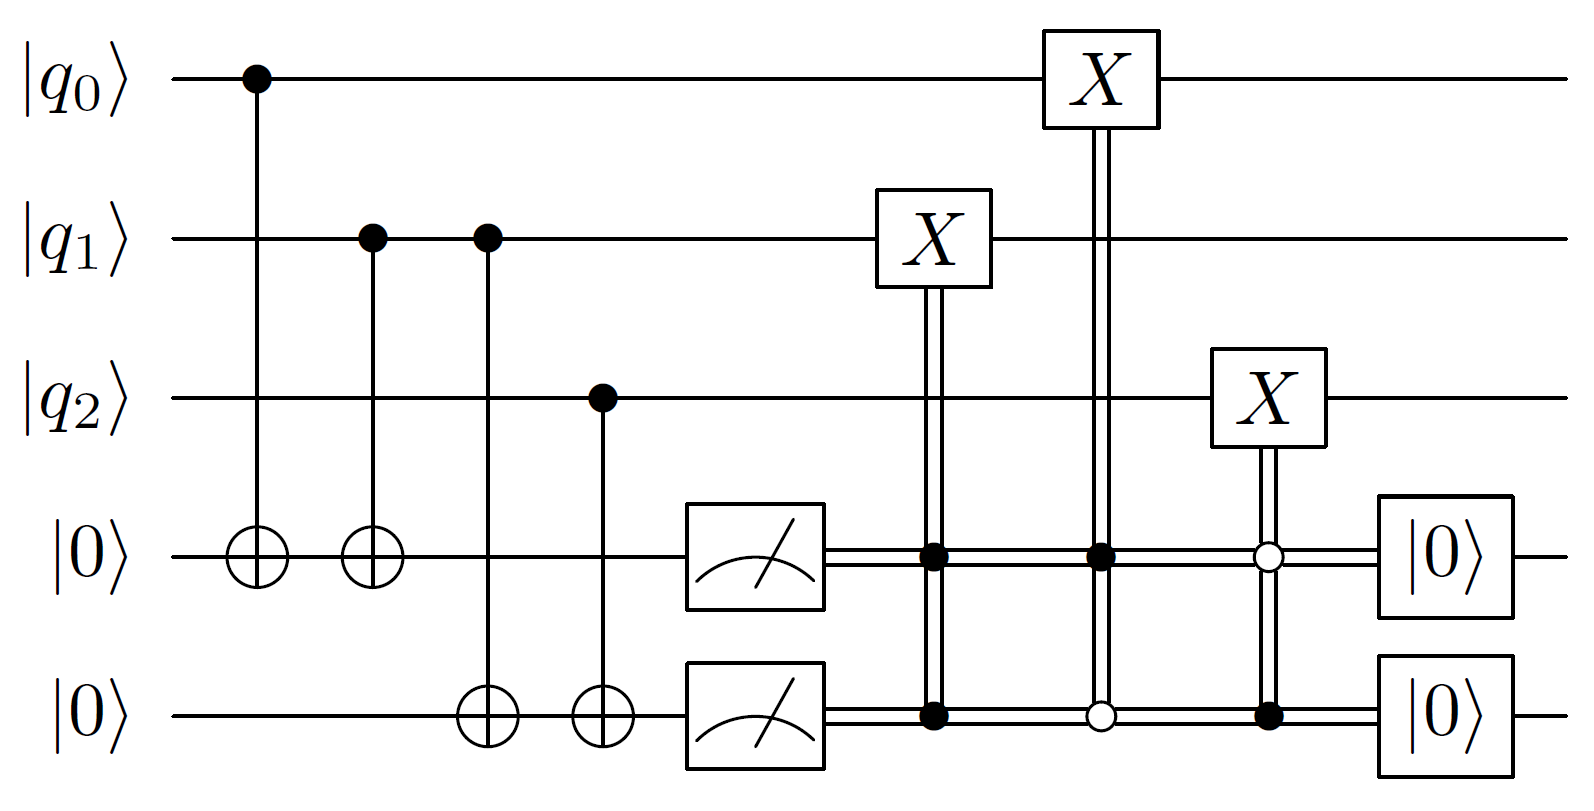
\includegraphics[scale=.25]{images/ErrorCorrection-BitFlipDetectionAndRecoveryCircuit.png}
    \caption{Bit flip detection and recovery circuit \cite{ThomasWong_2022}}
    \label{fig:BitFlipDetectionAndRecoveryCircuit}
\end{figure}

\section{Phase Flip Code}

Phase flip errors can similarly be corrected by using three physical qubits to encode a logical qubit. Since a complete phase flip error in the $\ket{+}$ and $\ket{-}$ basis switches between these states, logical qubits are the following:
$$\ket{0_L}=\ket{+++}$$
$$\ket{1_L}=\ket{---}$$
$$\ket{\psi}=\alpha\ket{0}+\beta\ket{1}  \underrightarrow{encode}  \ket{{\psi}_{L}}=\alpha\ket{0_L}+\beta\ket{1_L}$$

A circuit that performs this encoding is illustrated in figure \ref{fig:PhaseFlipEncodingCircuit}:

\begin{figure}[h!]
    \centering
    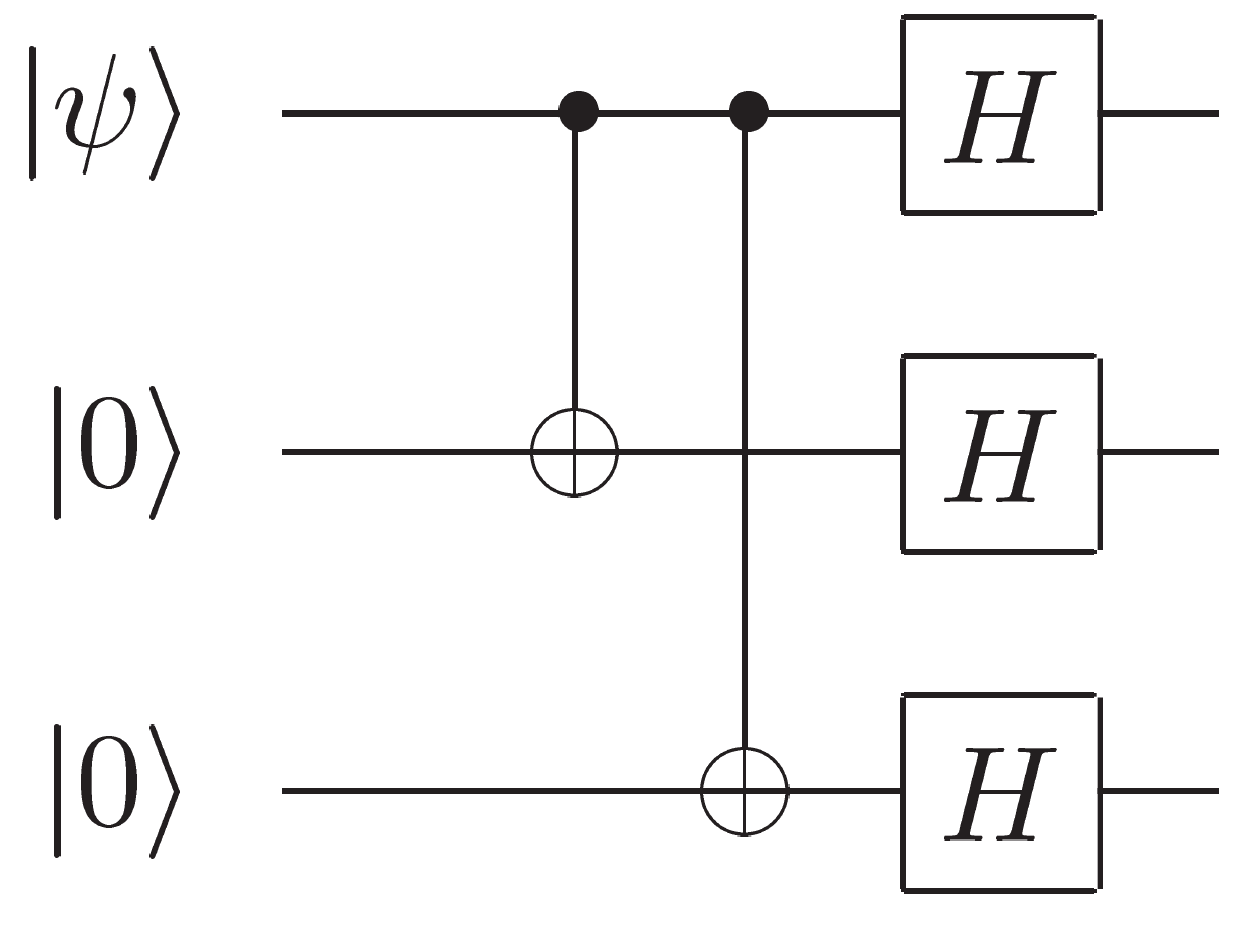
\includegraphics[scale=.25]{images/ErrorCorrection-PhaseFlipEncodingCircuit.png}
    \caption{Phase flip encoding circuit \cite{NielsenChuang_2012}}
    \label{fig:PhaseFlipEncodingCircuit}
\end{figure}

After the logical qubit has been manipulated, syndrome detection and recovery is done. Like in the bit flip case, there are four posibilities at this stage:
\begin{itemize}[noitemsep]
    \item No error: $\alpha\ket{+++}+\beta\ket{---}$
    \item First qubit flipped: $\alpha\ket{-++}+\beta\ket{+--}$
    \item Second qubit flipped: $\alpha\ket{+-+}+\beta\ket{-+-}$
    \item Third qubit flipped: $\alpha\ket{++-}+\beta\ket{--+}$
\end{itemize}

The circuit shown in figure \ref{fig:PhaseFlipDetectionAndRecoveryCircuit} detects the error using two auxiliary qubits that are entangled with the logical qubit such that measurements on those qubits yield two classical bits of information whose values map to a specific recovery operation that is then applied. In this case, instead of using the $X$ gate to correct errors, the $Z$ gate is used as the recovery operation for the qubit that was flipped.

\begin{figure}[h!]
    \centering
    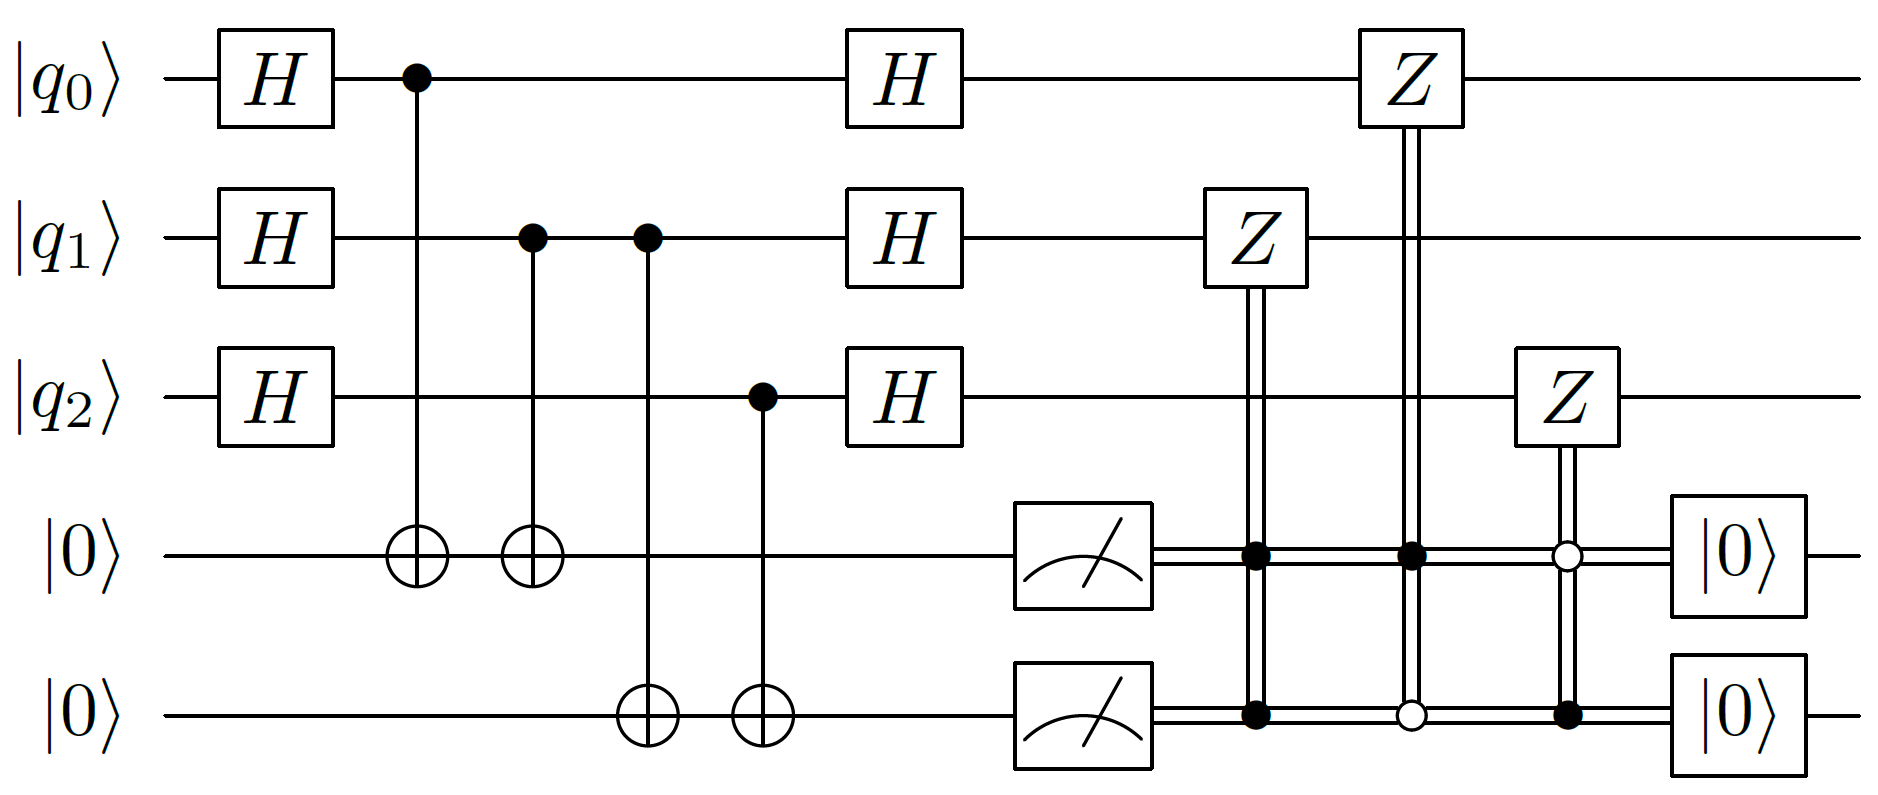
\includegraphics[scale=.25]{images/ErrorCorrection-PhaseFlipDetectionAndRecoveryCircuit.png}
    \caption{Bit flip detection and recovery circuit \cite{ThomasWong_2022}}
    \label{fig:PhaseFlipDetectionAndRecoveryCircuit}
\end{figure}

\section{Shor Code}

There is a quantum code which can protect against the effects of an arbitrary error on a single qubit knwon as the Shor code. The code is a combination of three qubit phase flip and bit flip codes. First, we encode the qubit using the phase flip code such that $\ket{0} \rightarrow \ket{+++}$ and $\ket{1} \rightarrow \ket{---}$. Next, we encode each one of these qubits using the three qubit bit flip code such that $\ket{+} \rightarrow \frac{\ket{000}+\ket{111}}{\sqrt{2}}$ and $\ket{-} \rightarrow \frac{\ket{000}-\ket{111}}{\sqrt{2}}$. This results in the following logical qubits:
$$\ket{0_L}=\frac{(\ket{000}+\ket{111})(\ket{000}+\ket{111})(\ket{000}+\ket{111})}{2\sqrt{2}}$$
$$\ket{1_L}=\frac{(\ket{000}-\ket{111})(\ket{000}-\ket{111})(\ket{000}-\ket{111})}{2\sqrt{2}}$$

A circuit that performs this encoding is illustrated in figure \ref{fig:ShorEncodingCircuit}:

\begin{figure}[h!]
    \centering
    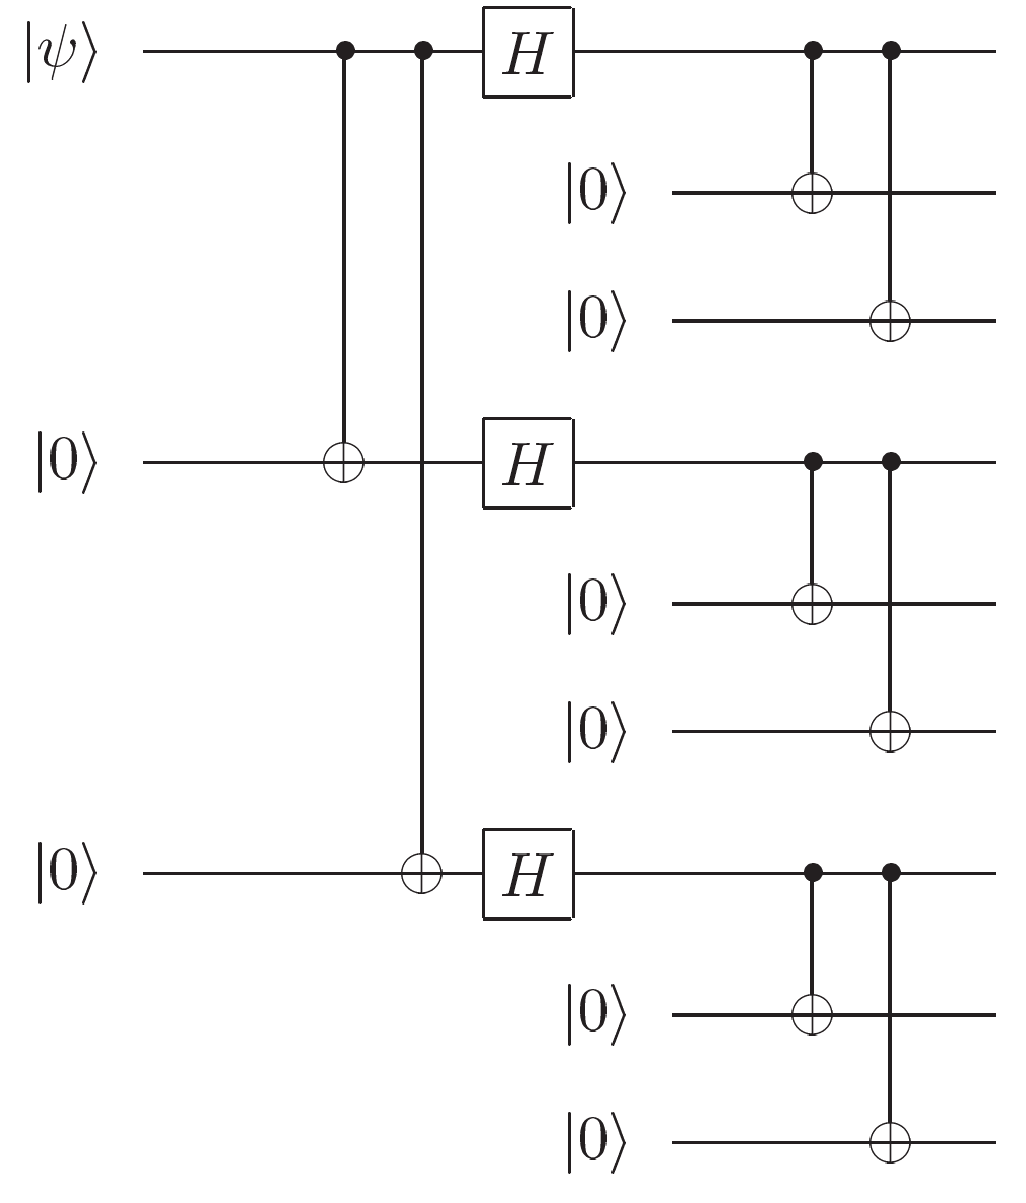
\includegraphics[scale=.25]{images/ErrorCorrection-ShorEncodingCircuit.png}
    \caption{Phase flip encoding circuit \cite{NielsenChuang_2012}}
    \label{fig:ShorEncodingCircuit}
\end{figure}

Syndrome detection and recovery for the Shor code is performed by combining bit flip and phase flip detection and recovery. Figure \ref{fig:ShorBitFlipDetectionAndRecoveryCircuit} shows bit flip detection and recovery. To do the same for phase flips we would just have to use the previously shown phase flip detection and recovery circuit on the first qubit of each bit flip encoded block.

\begin{figure}[h!]
    \centering
    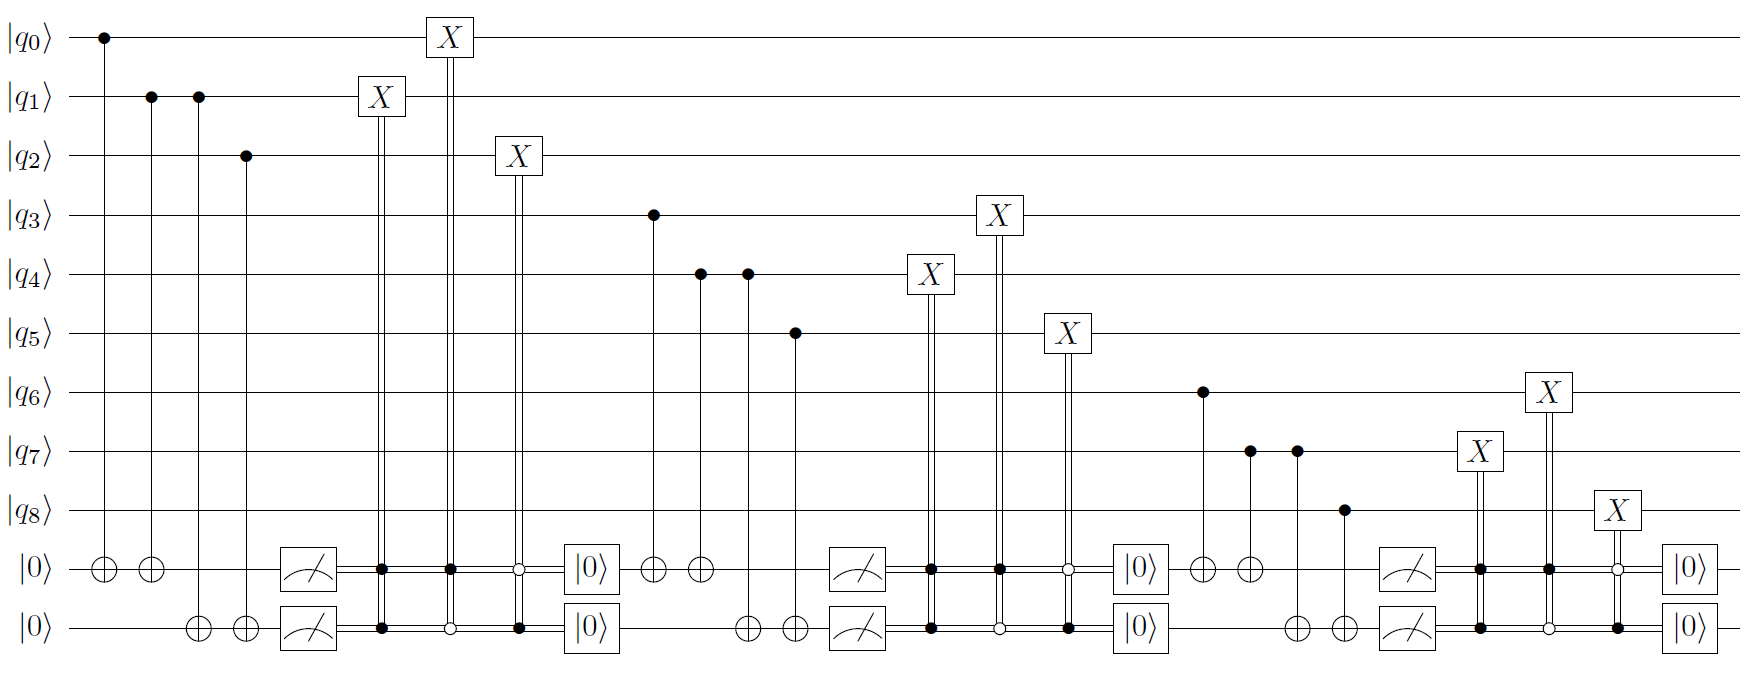
\includegraphics[scale=.35]{images/ErrorCorrection-ShorBitFlipDetectionAndRecoveryCircuit.png}
    \caption{Bit flip detection and recovery circuit on a Shor encoded qubit \cite{ThomasWong_2022}}
    \label{fig:ShorBitFlipDetectionAndRecoveryCircuit}
\end{figure}

Note that the Shor code corrects all quantum errors assuming each triplet experiences at most one bit flip error per correction cycle, and at most one triplet experiences a phase flip error per correction cycle.

\section{Quantum Error-Correction Without Measurement}

We have described quantum error-correction as a two stage process: a syndrome detection step that uses quantum measurement followed by a recovery step that applies unitary operations based on the results of the measurement. It is posible to perform error-correction using only unitary operations and auxiliary qubits prepared in standard states.

For example, figure \ref{fig:BitFlipDetectionAndRecoveryCircuitDelayedMeasurement} shows a delayed measurement circuits that perform syndrome detection and error recovery for bit flip errors:

\begin{figure}[h!]
    \centering
    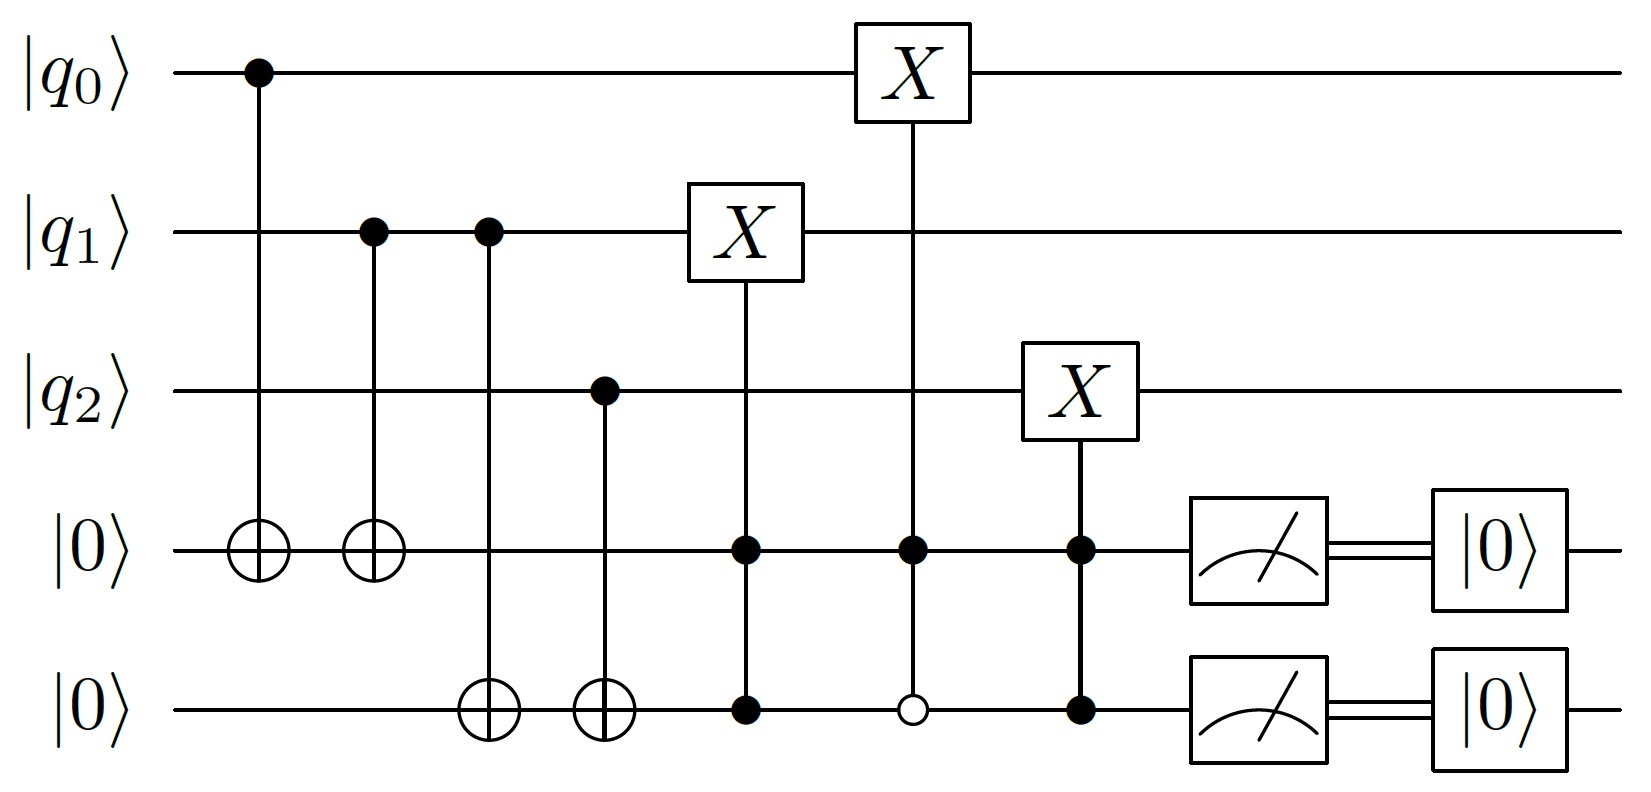
\includegraphics[scale=.25]{images/ErrorCorrection-BitFlipDetectionAndRecoveryCircuitDelayedMeasurement.png}
    \caption{Bit flip detection and recovery circuit using delayed measurement \cite{ThomasWong_2022}}
    \label{fig:BitFlipDetectionAndRecoveryCircuitDelayedMeasurement}
\end{figure}

The advantage this provides is that for some real-world quantum systems it is very difficult to apply different unitary operations based on quantum measurements so an alternate procedure is needed.

\section{Fault-Tolerant Quantum Computation}

One of the most useful applications of quantum error correction is the protection of quantum information as it dynamically undergoes computation. An arbitrary good quantum computation can be achieved provided only that the error probability per gate is below a certain constant threshold. A quantum computer that accumulates error slow enough that error can be corrected in called fault-tolerant.

The basic idea behind fault-tolerant quantum computation is to perform computations directly on encoded logical qubits such that decoding is never required.

Figure \ref{fig:FaultTolerantCircuit} shows a circuit using fault-tolerant logical operations. In this specific case, seven physical qubits are being used to encode and error-correct each logical qubit. One thing to note is that the reason the second error-correction step performed in the second qubit is that simply storing qubits for a period of time introduces errors and should periodically be error-corrected in order to prevent acumulation of errors.

\begin{figure}[h!]
    \centering
    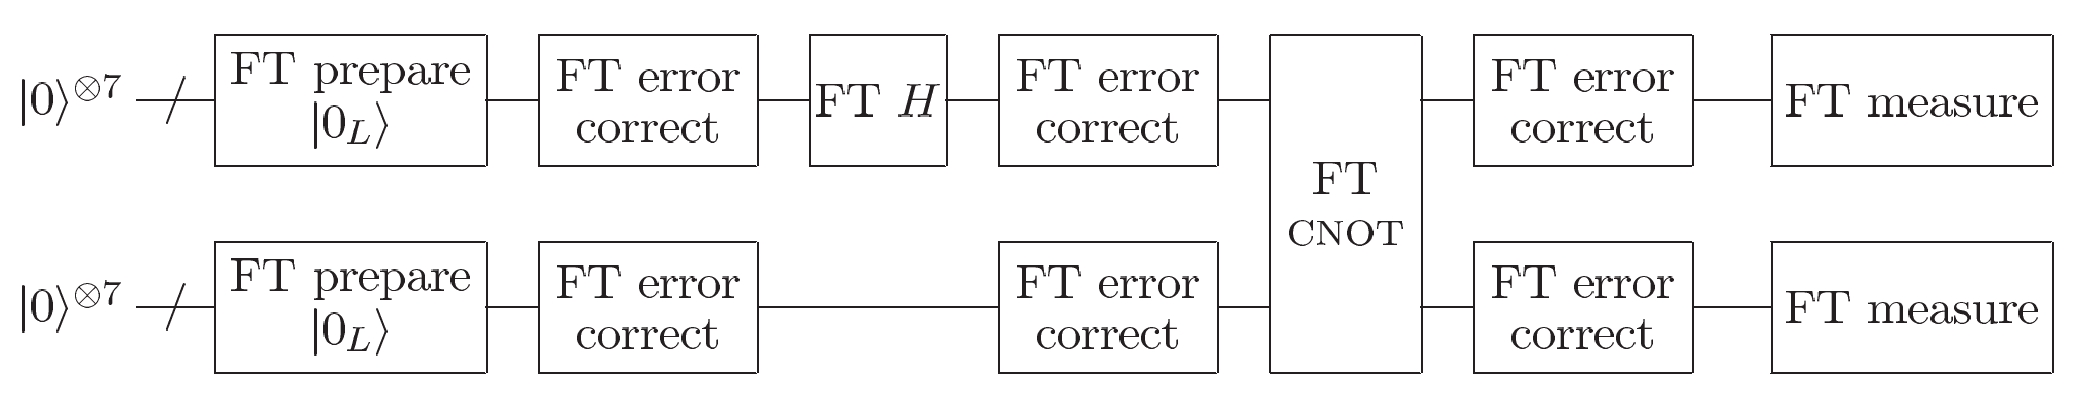
\includegraphics[scale=.30]{images/ErrorCorrection-FaultTolerantCircuit.png}
    \caption{Example of a fault-tolerant circuit \cite{NielsenChuang_2012}}
    \label{fig:FaultTolerantCircuit}
\end{figure}
